% The Proposal Boundary -- Santosh Kumar -- v0.1, October 2026
% Build: make   (or: pdflatex each figures/fig*.tex, then pdflatex this file twice)
\documentclass[10pt,letterpaper]{article}

\usepackage[T1]{fontenc}
\usepackage[utf8]{inputenc}
\usepackage{charter}
\usepackage[scaled=0.9]{helvet}
\usepackage[letterpaper,textwidth=6.0in,top=1.0in,bottom=1.1in]{geometry}
\usepackage{microtype}
\usepackage{graphicx}
\usepackage{xcolor}
\usepackage{enumitem}
\usepackage{titlesec}
\usepackage{caption}
\usepackage{fancyhdr}
\usepackage{fancyvrb}
\usepackage{pifont}
\usepackage[framemethod=default]{mdframed}
\usepackage[hidelinks]{hyperref}

\definecolor{ink}{RGB}{28,28,30}
\definecolor{muted}{RGB}{112,114,121}
\definecolor{accent}{RGB}{172,56,44}
\definecolor{panel}{RGB}{244,245,247}
\color{ink}

\hypersetup{
  pdftitle={The Proposal Boundary: Constraining the Interface Between Probabilistic Reasoning and Consequential Execution},
  pdfauthor={Santosh Kumar},
  pdfsubject={Agent runtime architecture},
  pdfkeywords={AI agents, authorization, runtime, proposal boundary}
}

% With a ragged bottom, LaTeX's negative penalties before headings and lists
% make it break pages early. Neutralise them so pages fill.
\makeatletter
\@secpenalty=0 \@beginparpenalty=0 \@endparpenalty=0 \@itempenalty=0
\makeatother
\renewcommand{\topfraction}{0.85}
\renewcommand{\bottomfraction}{0.7}
\renewcommand{\textfraction}{0.1}
\renewcommand{\floatpagefraction}{0.8}
\raggedbottom

\linespread{1.06}
\setlength{\parindent}{0pt}
\setlength{\parskip}{0.52em plus 0.1em minus 0.05em}
\frenchspacing

% headings
\titleformat{\section}{\sffamily\bfseries\fontsize{11.5}{14}\selectfont}{\thesection}{0.7em}{}
\titlespacing*{\section}{0pt}{1.35em plus 0.3em}{0.3em}
\newcommand{\run}[1]{\textbf{#1}\hspace{0.45em}}

% captions
\captionsetup{font={small,sf},labelfont={bf},labelsep=period,justification=raggedright,
  singlelinecheck=false,skip=7pt}

% running footer
\pagestyle{fancy}
\fancyhf{}
\renewcommand{\headrulewidth}{0pt}
\fancyfoot[L]{\sffamily\fontsize{7.5}{9}\selectfont\color{muted}The Proposal Boundary \textperiodcentered\ v0.1 \textperiodcentered\ October 2026}
\fancyfoot[R]{\sffamily\fontsize{7.5}{9}\selectfont\color{muted}\thepage}

% monospace: OT1 Computer Modern Typewriter (Type 1 everywhere)
\newcommand{\code}[1]{{\fontencoding{OT1}\fontfamily{cmtt}\selectfont #1}}

% a statement set apart from the text
\newmdenv[topline=false,bottomline=false,rightline=false,linewidth=1.6pt,linecolor=accent,
  innerleftmargin=11pt,innerrightmargin=0pt,innertopmargin=1pt,innerbottommargin=1pt,
  skipabove=0.75em,skipbelow=0.45em,leftmargin=0pt,rightmargin=0pt]{keyline}

% terminal excerpt
\newmdenv[linewidth=0.4pt,linecolor=muted!55,backgroundcolor=panel,
  innerleftmargin=9pt,innerrightmargin=6pt,innertopmargin=6pt,innerbottommargin=6pt,
  skipabove=0pt,skipbelow=0pt,leftmargin=0pt,rightmargin=0pt]{terminal}

\setlist[description]{leftmargin=1.9em,labelindent=0pt,labelwidth=1.4em,labelsep=0.5em,
  itemsep=0.35em,topsep=0.3em,parsep=0pt,font=\sffamily\bfseries\small\color{accent}}

\begin{document}

%% ---------------------------------------------------------------- title
{\sffamily
{\fontsize{23}{27}\selectfont\bfseries The Proposal Boundary\par}
\vspace{0.5em}
{\fontsize{12.5}{16}\selectfont Constraining the Interface Between Probabilistic Reasoning\\
and Consequential Execution\par}
\vspace{1.1em}
{\fontsize{10}{13}\selectfont \textbf{Santosh Kumar}\hspace{0.9em}{\color{muted}October 2026 \textperiodcentered\ v0.1}\par}
}
\vspace{0.9em}
{\color{accent}\hrule height 1.6pt}
\vspace{1.0em}

%% ------------------------------------------------------------- abstract
{\sffamily\bfseries\small Abstract}\hspace{0.6em}%
AI agents are usually built by giving a language model a set of tools and letting it call them
from inside its reasoning loop. In that design, deciding that something should happen and
causing it to happen are one event. This note describes a different interface, the
\emph{proposal boundary}. The model holds no authority to cause effects. Its only output is a
proposal: a value in a small language that names the operations it wants performed, the claims
it makes about their outcome, and the evidence by which each claim can be checked. A proposal
exists independently of its execution, so the runtime can validate it, obtain
authorization for it, apply it, and check its claims against what the runtime itself observed.
The note defines the boundary, describes Current, a runtime that implements it for changes to
software projects, and states what the design leaves unsolved.

%% ====================================================================
\section{Reasoning and authority are coupled}

The common agent architecture is a loop. A model receives a task and emits a tool call; the
call is executed; its result is appended to the model's context; the model continues until it
decides it is done (Figure~\ref{fig:boundary}a). The loop is simple and it works, which is why
most agent frameworks are built on it.

Its defining property is that each tool call is a decision and an act at once. Three
consequences follow.

\run{Nothing exists to authorize.} Before the first effect there is no description of the
work as a whole, only the next call. A person or a policy asked to approve can approve one
step at a time, without knowing what the steps add up to.

\run{What the system might do is a fact about the model.} The possible behaviours are the
sequences of tool calls the model might emit, a set that grows with every tool added and every
additional step. An argument that the system is safe has to be an argument about what a
stochastic process will not do.

\run{The record is the transcript.} What the model reported and what occurred are interleaved
in one stream, and the report tends to be read as the result. ``All tests pass'' in a final
message is a sentence the model wrote.

Confirmation prompts gate one call at a time. Allowlists and sandboxes limit which calls can
succeed and what they can reach. All three are worth having. None of them produces a
description of the intended work that exists before the work begins.

\begin{figure}[!b]
\centering
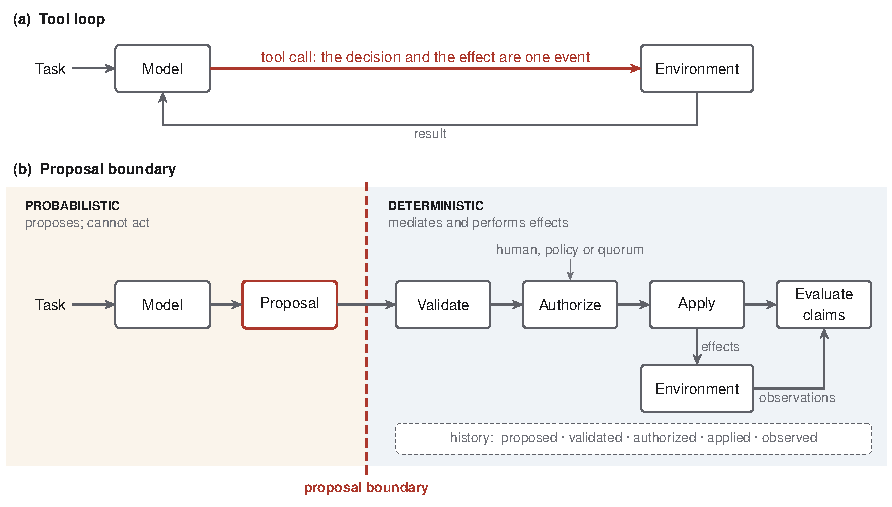
\includegraphics[width=0.94\textwidth]{figures/fig1-boundary.pdf}
\caption{(a) In a tool loop the model's output is the effect. (b) Behind a proposal boundary
the model's output is a proposal, and every later step is carried out by the
runtime, not by the model that wrote the proposal.}
\label{fig:boundary}
\end{figure}

%% ====================================================================
\section{The proposal boundary}

A proposal boundary is an interface between a probabilistic reasoner and the environment it
acts on. It has four properties.

\begin{description}
\item[P1] \textbf{No ambient authority.} The reasoner cannot cause effects. It holds no tools
  that act on the environment. Its only output is a proposal.
\item[P2] \textbf{A bounded language.} A proposal is a value in a language of operations that
  the runtime defines and understands. Output that does not decode into it is not a proposal
  and goes no further.
\item[P3] \textbf{Independent existence.} A proposal exists before its execution and apart
  from it. It can be stored, read, validated, authorized, rejected, or never applied.
\item[P4] \textbf{Outcomes belong to the runtime.} Whether an operation happened, and whether
  a claim about it held, is established by what the runtime observed, never by what the
  reasoner reported.
\end{description}

Figure~\ref{fig:boundary}b shows the result. Everything left of the boundary proposes.
Everything right of it mediates and performs effects.

\begin{keyline}
\itshape The agent decides what should happen. The runtime decides what may happen and
establishes what did.
\end{keyline}

``Deterministic'' needs care. Effects are not deterministic: a test suite can pass on one run
and fail on the next. What is deterministic is the runtime's handling of a proposal. Given the
same proposal, the same authorization and the same observations, it makes the same decisions.

%% ====================================================================
\section{The proposal as an intermediate representation}
\label{sec:ir}

A proposal contains an ordered list of requested operations; claims about what those
operations will achieve; for each claim, an evidence specification that names the operation
whose result will be observed and the condition that result must satisfy; and a justification
written for a reviewer, which the runtime stores and does not interpret.

It would be easy to read this as an approval dialog with more detail in it. A closer
comparison is the intermediate representation in a compiler, which exists so that several
independent passes can work on one object. A proposal is read by a validator that checks it
against the rules of the environment, by a reviewer or a policy that decides whether to
authorize it, by an executor that applies it, and afterwards by anyone comparing what was
requested with what occurred. None of these needs the model, its prompt or its reasoning.
Each needs only the proposal.

The model's output is untrusted input, and turning it into a proposal is parsing: a fixed set
of operation kinds, required fields, and references that must resolve. What matters about the
language is less which operations it contains than that it is smaller and more regular than
the environment the model reasons about.

A bounded language does not by itself bound effects. If the language includes an operation as
expressive as ``run this command,'' the set of well-formed proposals is still enumerable in
form, but what one such operation can do is not. The boundary makes that operation visible
before it runs and attributable after. It does not limit what the command can reach. That is
a sandbox's job, and the two compose: the boundary governs what is requested, the sandbox
governs what an operation can touch.

%% ====================================================================
\section{Authorization is not execution}

\begin{figure}[!t]
\centering
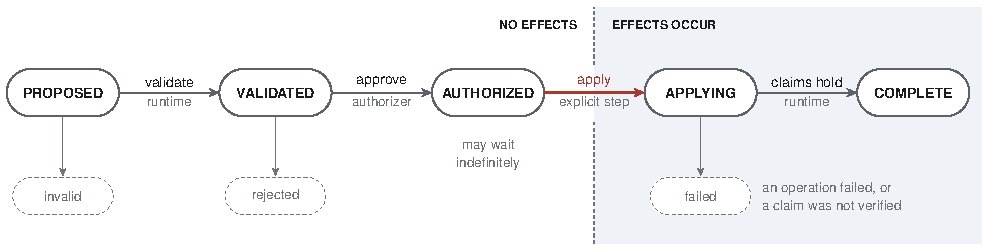
\includegraphics[width=\textwidth]{figures/fig2-lifecycle.pdf}
\caption{The lifecycle of a proposal. Authorization and application are separate transitions,
and no effect occurs before the second.}
\label{fig:lifecycle}
\end{figure}

A proposal moves through the states in Figure~\ref{fig:lifecycle}. The transition this
section is about is the one between \emph{authorized} and \emph{applying}.

\begin{keyline}
\itshape Approval changes the authorization state of a proposal. It causes no effects.
\end{keyline}

Applying is a separate act and is recorded separately. The separation does four things.

It lets the authorizer change without the executor changing. A person, a policy, a second
model or a quorum can each move a proposal to \emph{authorized}; the runtime's obligation, to
apply only what has been authorized, is the same in every case.

It ties authorization to one immutable object. A revised proposal is a different proposal and
needs its own authorization.

It makes room for time. Authorization can arrive minutes or days after validation, and the
environment can change in between. Validity is therefore checked twice: once so that nobody is
asked to approve something that could never be allowed, and again at application, against the
environment as it then stands. An authorized proposal can still fail to apply.

It lets the history answer four questions separately: what was requested, who authorized it
and when, what was applied, and what was observed.

%% ====================================================================
\section{Claims are not results}

When an agent ends its work with ``the test suite passes,'' it has made a claim. In a tool
loop nothing distinguishes that claim from a result.

Behind a proposal boundary a claim is part of the proposal and has a defined form: a statement
and an evidence specification. The specification names an operation in the same proposal and a
condition on its result; for example, the operation runs the test command and the condition
is that its exit status is zero. The runtime applies the operation, records what it observed,
evaluates the condition, and records the claim as verified or not verified together with the
observation (Figure~\ref{fig:claims}). A claim that does not hold stops the proposal. Later
operations are not applied, and the observation that disproved the claim stays in the history.

\begin{keyline}
\itshape The actor that proposes the work is not the authority that declares it successful.
\end{keyline}

\begin{figure}[!t]
\centering
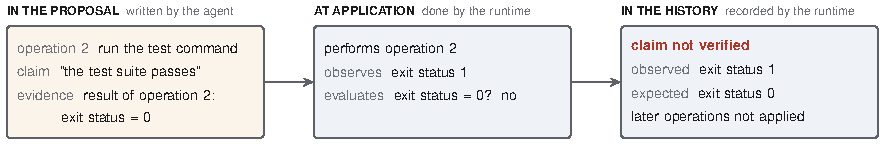
\includegraphics[width=\textwidth]{figures/fig3-claims.pdf}
\caption{A claim that fails. The agent supplies the statement and says how it can be checked;
the runtime makes the observation and records the outcome.}
\label{fig:claims}
\end{figure}

This has two limits. First, the agent still writes the evidence specification. The runtime
establishes that the observation satisfied the stated condition, not that the condition is a
good test of the statement: a passing suite says nothing about whether the new behaviour is
tested. But the check is in the proposal, so its adequacy can be judged at review, before
anything runs. Second, a statement with no evidence specification remains an assertion. It
should be shown to a reviewer as one and never recorded as verified.

%% ====================================================================
\section{What the boundary changes}

A tool-loop agent poses the question: what might this model do, with these tools, over this
many steps? The subject of that question is a model. A proposal-bound agent poses a different
one: what can be said in the proposal language, and what does the runtime do with each thing
that can be said? The subject is a language and a program, both written by the system's
builder, both open to being read, tested and changed.

That is the sense in which the possibility space shrinks. The model is no less capable of
reaching a bad conclusion. But a bad conclusion arrives as a proposal, a finite object that
can be refused, and not as an effect.


%% ====================================================================
\section{Current}

Current is an experimental runtime built to test whether this boundary is practical. It works
on software projects. Its source is not public, and this section describes its behaviour, not
its design.

A task is submitted against a project directory. The runtime assembles a snapshot of the
project and calls the model once, with no tools. The model's reply is stored unmodified and
then decoded. A reply that names an unknown operation, omits a required field, or contains a
reference that does not resolve produces no proposal. A decoded proposal is validated before
anyone is asked to approve it: every path it names must lie inside the project, and each claim
must cite an earlier operation capable of producing the observation the claim depends on.

Current has two modes. In \emph{plan} mode the workflow ends once the proposal is validated,
and that proposal can never be authorized or applied. In \emph{apply} mode the workflow stops
and waits. Figure~\ref{fig:terminal} shows that point for a task that adds rate limiting to a
login endpoint.

\begin{figure}[!ht]
\begin{terminal}
\begin{Verbatim}[commandchars=\\\{\},formatcom=\fontencoding{OT1}\fontfamily{cmtt}\fontsize{7.15}{9.7}\selectfont]
  Claims
    - The login endpoint is rate limited per client IP using the existing lib/rateLimit.ts helper.
    - Requests exceeding 5 login attempts per 60 seconds receive a 429 response with a Retry-After header.
    - The existing test suite should continue to pass.

{\normalfont\ding{51}} Proposal decoded
{\normalfont\ding{51}} Proposal validated

MODE: APPLY
0 effects executed.

Waiting for approval. Nothing has been applied.
  current review sha256:8c48adf23aa9
  current approve sha256:8c48adf23aa9 [-m <message>]
\end{Verbatim}
\end{terminal}
\caption{Excerpt of Current's terminal output after it has produced and validated a proposal
in apply mode. The claims are statements about an outcome that does not exist yet. No
operation has run.}
\label{fig:terminal}
\end{figure}

Approving and applying are separate commands and separate entries in the history. An approved
proposal stays approved and unapplied until it is applied. At application the runtime checks
each operation against the project boundary again, immediately before performing it, with the
filesystem as it then stands. It performs the operations in order, records each result, and
evaluates each claim against the recorded result of the operation the claim cites.

Every step is an entry in an append-only history: the task, the proposal, its validation, the
decision, each effect and each claim result. A workflow's state is computed from that history
and from nothing else, so it can be recomputed at any time. Recomputing state does not
re-execute effects. If the runtime stops while applying a proposal, it does not resume or
retry on restart. It marks the workflow failed and records that effects may have run without
a completion record.

%% ====================================================================
\section{Limitations}

\run{Observation.} A looping agent learns as it goes: it reads a file, runs a command, and
adjusts. Behind a proposal boundary a read is an operation like any other, so whatever the
reasoner needs to see must come either from context the runtime assembles in advance or from
applying one proposal and proposing again. Current does only the first: one proposal for each
task, from a snapshot. That is enough for changes whose shape can be worked out by reading the
code. It is not enough for work that has to run things to find out what to do. Proposing in
rounds, with a policy that authorizes read-only proposals automatically, is the natural
extension. What it costs in latency, and how its capability compares with a loop, has not been
measured.

\run{Expressive operations.} As Section~\ref{sec:ir} said, the boundary does not confine an operation
that can do anything. Current's command operation runs in the project directory and is not
otherwise confined.

\run{Review.} A person asked to approve every proposal will soon approve by habit. The
boundary gives a policy something to evaluate. It does not supply the policy.

\run{Atomicity.} A proposal is applied one operation at a time and is not a transaction. If
the fourth of six operations fails, the first three remain applied. Current records the prior
contents of the files it changes but does not roll back.

\run{Evaluation.} This note makes an argument and reports an implementation. It contains no
measurement of task success, cost or review burden against a tool-loop baseline.

%% ====================================================================
\section{Related work}

The boundary applies old ideas to a new kind of untrusted subject. A reference
monitor~\cite{anderson72} mediates every access through a mechanism that is tamperproof,
always invoked, and small enough to analyse. The principle of least
privilege~\cite{saltzer75} gives a subject only the authority its task requires. A model with
tools holds standing authority. A model behind a strict proposal boundary holds no direct
authority to cause effects.

Infrastructure tools separate planning from applying: a plan is computed, shown, and applied
as a distinct step~\cite{terraform}. There the planner is deterministic and trusted. Here the
planner is the untrusted component, which is why the plan language is also the trust boundary
and why the plan carries claims to be checked. The planning modes of coding agents typically
produce prose for a person, and what executes afterwards is the tool loop, not the plan.

In proof-carrying code~\cite{necula97} an untrusted producer attaches a proof that the host
checks before running the code. An evidence specification is much weaker, an observation to
make and not a proof, but it assigns the roles the same way: the producer says how its claim
can be checked and the host does the checking.

The Dual LLM pattern~\cite{willison23} and CaMeL~\cite{debenedetti25} separate the component
that plans from the component exposed to untrusted data; CaMeL runs the plan in an interpreter
that tracks where data came from and enforces policies when tools are called. Their target is
prompt injection. The proposal boundary is concerned with authority more generally and treats
the plan as a durable object with its own authorization lifecycle. The approaches are
compatible.

%% ====================================================================
\section{Conclusion}

Nothing in the boundary is specific to code. It applies wherever effects can be named in a
bounded vocabulary: infrastructure changes, database mutations, payments, calls to external
services. Current demonstrates it for software projects only, and only for a single round of
proposing.

Agents will get better at reasoning. That is a reason to give their reasoning more room, not
a reason to give it more authority.

\begin{keyline}
\itshape Reason broadly. Propose narrowly. Execute under deterministic control.
\end{keyline}

%% ====================================================================
\begingroup
\small
\renewcommand{\refname}{References}
\begin{thebibliography}{9}
\setlength{\itemsep}{0.25em}

\bibitem{anderson72} J.~P. Anderson. \emph{Computer Security Technology Planning Study}.
  ESD-TR-73-51, U.S. Air Force Electronic Systems Division, 1972.

\bibitem{saltzer75} J.~H. Saltzer and M.~D. Schroeder. The protection of information in
  computer systems. \emph{Proceedings of the IEEE}, 63(9):1278--1308, 1975.

\bibitem{terraform} HashiCorp. Terraform documentation: \code{terraform plan} and
  \code{terraform apply}.

\bibitem{necula97} G.~C. Necula. Proof-carrying code. In \emph{Proceedings of the 24th ACM
  Symposium on Principles of Programming Languages (POPL)}, 1997.

\bibitem{willison23} S.~Willison. The Dual LLM pattern for building AI assistants that can
  resist prompt injection. \mbox{simonwillison.net}, April 2023.

\bibitem{debenedetti25} E.~Debenedetti et al. Defeating prompt injections by design. arXiv
  preprint, 2025.

\end{thebibliography}
\endgroup

\end{document}
